\section{Method}
We begin by outlining preliminaries on Gaussian Splatting and planar depth rendering. \Cref{sec:pgsr_modifications} details modifications to PGSR for sparse settings, followed by our dense initialization strategy in \Cref{sec:dense_initialization}. We then present our uncertainty-aware Pearson loss in \Cref{sec:depth_supervision} and artifact-free normal supervision in \Cref{sec:normal_supervision}. Finally, \Cref{sec:depth_warping} describes our depth warping approach for improving view consistency.

\subsection{Preliminaries}

\paragraph{Gaussian Splatting.}
\textit{3D Gaussian Splatting} (3DGS) introduced by Kerbl et al.~\cite{3dgs2023} achieves great novel view synthesis results with high efficiency by leveraging a Gaussian scene representation. Another improvement of this scene representation over NeRF is the real-time rendering speed, as well as much faster training times. Our approach also builds upon 3DGS.
The scene representation is defined by a set of 3D Gaussians.
Each Gaussian can be defined by a 3D covariance matrix $\Sigma \in \mathbb{R}^{3 \times 3}$ and the 3D center point $\mu \in \mathbb{R}^3$ in world space,
\begin{equation}
    G(x) = e^{-\frac{1}{2}(x - \mu_i)^T\Sigma^{-1}(x - \mu_i)}.
\end{equation}

To project this 3D Gaussian onto the 2D image plane for rendering, the covariance matrix $\Sigma'$ in clip space is defined as the following:
\begin{equation}
    \Sigma' = J W \Sigma W^T J^T,
\end{equation}
where $J$ is the Jacobian of the affine approximation for this projection transformation and $W$ is the view transformation matrix.

For the covariance matrix to be physically meaningful, it needs to be positive semi-definite.
To ensure this throughout the training process, $\Sigma$ is defined as the following:
\begin{equation}
    \Sigma = R S S^T R^T,
\end{equation}
where $S \in \mathbb{R}^{3\times 3}$ is the scaling matrix, and $R \in \mathbb{R}^{3\times 3}$ is the rotation matrix.
This allows separate optimization of rotation and scaling and ensures that $\Sigma$ is positive semi-definite. For increased memory efficiency, the rotation matrix is stored as a quaternion, and scaling as 3D vector.

Furthermore, for rendering the color $C$, we blend the colors of each Gaussian along the ray, as follows:
\begin{equation}
    C = \sum^N_{i=1} T_i \alpha_i c_i,
\end{equation}
where $N$ is the number of Gaussians along a ray, $c_i$ is the color of the i-th Gaussian represented by spherical harmonics (SH) to account for view dependent effects, $\alpha_i$ is the weighted opacity of the i-th Gaussian and $T_i$ is the transmittance of the i-th Gaussian~\cite{3dgs2023}.

Transmittance $T_i$ is defined as:
\begin{equation}
\label{eq:transmittance}
    T_i = \prod^{i-1}_{j=1}(1 - \alpha_j).
\end{equation}%TODO, rewrite opacity
%where $\alpha_j$ is the weighted opacity of the j-th Gaussian~\cite{Catacaustics}.
By calculating the color for each ray from the camera, we can render an image.
The training of this Gaussian representation is done by back propagation with the following loss function:
\begin{equation}
    \mathcal{L} = (1 - \lambda) \mathcal{L}_1 + \lambda \mathcal{L}_{D-SSIM},
\end{equation}
where $\mathcal{L}_1$ is a simple $l_1$ loss between the rendered and ground-truth image and $\mathcal{L}_{D-SSIM}$ is an image similarity measure between rendered and ground-truth image~\cite{3dgs2023, dssim}.
3DGS relies on camera poses and points obtained from structure from motion (SfM). However, in sparse-view settings, the resulting point cloud can be highly sparse, and the overlap between the images may be insufficient to extract reliable structures or accurate camera poses. This leads to a challenging starting point for 3DGS optimization.

\paragraph{Depth and Normal Rendering.}
We use \textit{Planar-based Gaussian Splatting for Efficient
and High-Fidelity Surface Reconstruction}~\cite{pgsr2024} (PGSR) for normal and depth rendering. PGSR builds upon 3DGS, enabling the rendering and backpropagation of both the depth and normals.
A naive approach of computing the depth $D$ of a pixel would be to use depth accumulation defined as:
\begin{equation}
    D = \sum_{i=1}^N T_i \alpha_i z_i,
\end{equation}
where $T_i$ is the same as in ~\cref{eq:transmittance}, $\alpha_i$ is the weighted opacity of the i-th Gaussian and $z_i$ is its distance from the camera~\cite{gaussianproDepth}.
PGSR on the other hand compresses the 3D Gaussians to get flat 2D planes, from which unbiased depth and normal maps can be rendered~\cite{pgsr2024}.

To get the 2D planes, PGSR flattens the 3D Gaussians by minimizing the minimum scale and therefore defining the scale loss $\mathcal{L}_s$ as following:
\begin{equation}
    \mathcal{L}_s = ||\min(s_1, s_2, s_3)||_1,
\end{equation}
where $s_i$ is the i-th scale component of each Gaussian.

The direction of the minimum scale factor corresponds to the normal $n_i$.
Therefore, the normals per ray, $\mathcal{N}$, can be rendered as following:
\begin{equation}
    \mathcal{N} = \sum_{i=1}^N R_c^T n_i \alpha_i T_i,
\end{equation}
where $R_c$ is the rotation from the camera to the global world.%, $\alpha_i$ and $T_i$ is the same as in \cref{eq:transmittance}.

The distance $d_i$ from the Gaussian plane to the camera center is defined as:
\begin{equation}
    d_i = (R_c^T (\mu_i - T_c)) R_c^T n_i^T,
\end{equation}
where $T_c$ is the camera center in the world and $\mu_i$ is the center of the i-th Gaussian.

The distance $D$ along a ray can now be defined as:
\begin{equation}
    D = \sum_{i=1}^N d_i \alpha_i T_i.
\end{equation}
PGSR extends 3DGS by introducing an Image Edge-Aware Single-View Loss $\mathcal{L}_{svgeo}$, which optimizes the Gaussian Scene with the Local Plane Assumption. This assumption states that two neighbouring pixels can be considered as an approximate local plane, but only if these pixels do not belong to an edge. The loss helps to improve the local depth and normal consistency. They also propose a Multi-View Geometric Consistency Loss, $\mathcal{L}_{mvgeom}$, which enhances geometric smoothness by projecting the depth and normals from one frame to another. Finally, they employ a Multi-View Photometric Consistency Loss, $\mathcal{L}_{mvrgb}$, which projects the grayscale image from one camera to another camera through depth warping~\cite{pgsr2024}.

\subsection{PGSR Sparse-View}
\label{sec:pgsr_modifications}
Default PGSR does not work well for the sparse-view setting out-of-the-box because of the multi-view observer trim, which assures that each point is observed by multiple cameras and this is not guaranteed in sparse-view settings. Therefore, we deactivate this trimming for our method.
Another parameter that requires adjustment is the opacity reset interval. When opacity reset happens, fine details in the background will be lost and artifacts appear, as can be seen in \cref{fig:opacity_reset_example}. The details in \cref{fig:opacity_reset} at the back wall are completely lost and artifacts in the window frame become visible. By continuing the training process even further, the artifacts' strength increases, and they become even more prominent. When deactivating opacity reset, the background details are retained and the artifacts vanish without sacrificing the overall quality. This can also be seen in \cref{fig:no_opacity_reset}. The improvement is also reflected in the PSNR (Peak Signal-to-Noise Ratio), which increases from \textit{22.76} to \textit{23.73}.
With these few settings, it is already possible to run the PGSR framework with acceptable results. For improved performance, we deactivate the splitting strategy as it is not needed for our dense point cloud initialization. The point cloud is already very detailed and this setting does not improve the final results (\textit{cf.} \cref{tab:ablation}).

\begin{figure}
\centering
\begin{subfigure}{.24\textwidth}
    \centering
    \captionsetup{justification=centering, width=0.9\textwidth}
    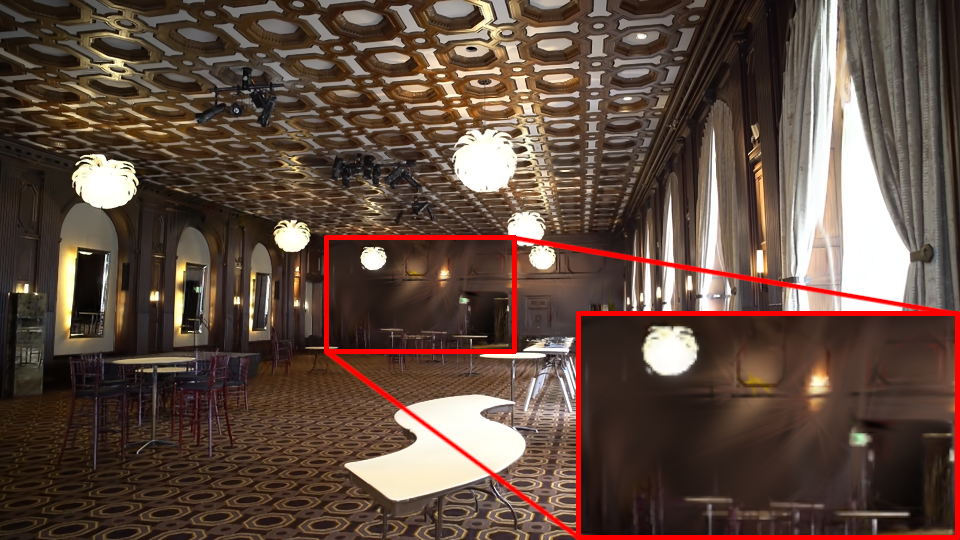
\includegraphics[width=0.98\linewidth]{figures/opacity_reset_ballroom_cutout.png}
    \caption{Ballroom scene with opacity reset.}
    \label{fig:opacity_reset}
\end{subfigure}%
\begin{subfigure}{.24\textwidth}
    \centering
    \captionsetup{justification=centering, width=0.9\textwidth}
    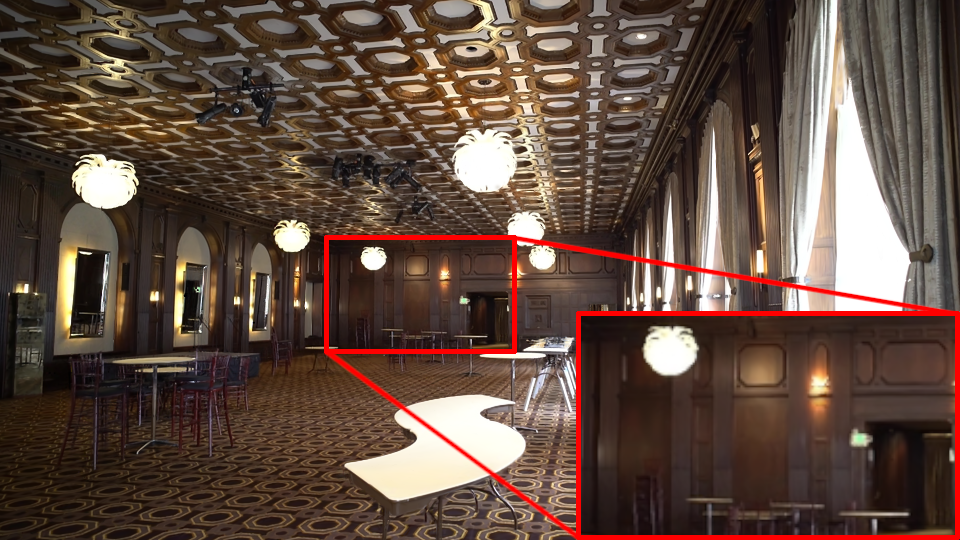
\includegraphics[width=0.98\linewidth]{figures/no_opacity_reset_ballroom_cutout.png}
    \caption{Ballroom scene without opacity reset.}
    \label{fig:no_opacity_reset}
\end{subfigure}
\caption{Comparison of the Ballroom scene from Tanks and Temples with and without opacity reset~\cite{tankstemples}. Background details are lost when opacity reset is executed, and image quality further degrades over the training process.}
\label{fig:opacity_reset_example}
\end{figure}

\subsection{Dense Initialization}
\label{sec:dense_initialization}
Sparse-view settings pose a fundamental challenge for standard SfM frameworks like COLMAP~\cite{SFM-Original, MVSPixel}, where limited image overlap can lead registration to fail. Furthermore, the resulting sparse point clouds serve as a poor initialization for 3DGS, complicating the optimization of Gaussian primitives and compromising geometric fidelity. To mitigate this, we leverage a pre-trained feed-forward network to predict both depth and camera parameters. This strategy provides the dense geometric initialization and accurate poses required for high-quality sparse-view reconstruction.
\Cref{fig:pointcloud_pi3} illustrates the point cloud generated by the feed-forward model $\pi^3$~\cite{wang2025pi3}, while \cref{fig:pointcloud_colmap} depicts the result from COLMAP~\cite{SFM-Original}. Both methods use the same 24 input views from the "bicycle" scene of the MipNeRF360 dataset~\cite{mipnerf360}, rendered here from an identical viewpoint. The difference in density is significant: The COLMAP reconstruction contains only 1,028 points, whereas $\pi^3$ yields 1,013,106 points. Note that the $\pi^3$ output was filtered using the default confidence threshold of 20\%.
\begin{figure}
\centering
\begin{subfigure}[t]{.25\textwidth}
  \centering
  \captionsetup{justification=centering}
  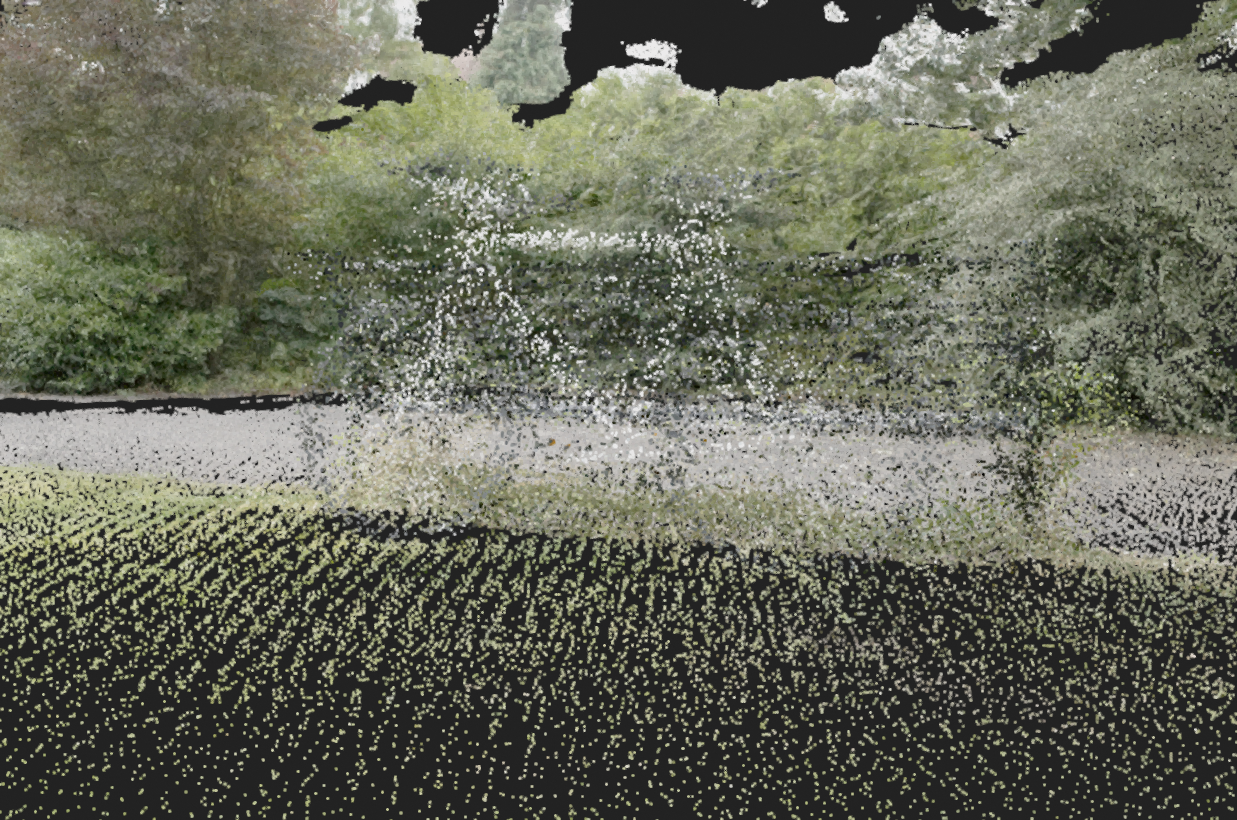
\includegraphics[width=0.98\linewidth]{figures/pi3_pointlcoud.png}
  \caption{Point cloud inferred with $\pi^3$.}
  \label{fig:pointcloud_pi3}
\end{subfigure}%
\begin{subfigure}[t]{.25\textwidth}
  \centering
  \captionsetup{justification=centering}
  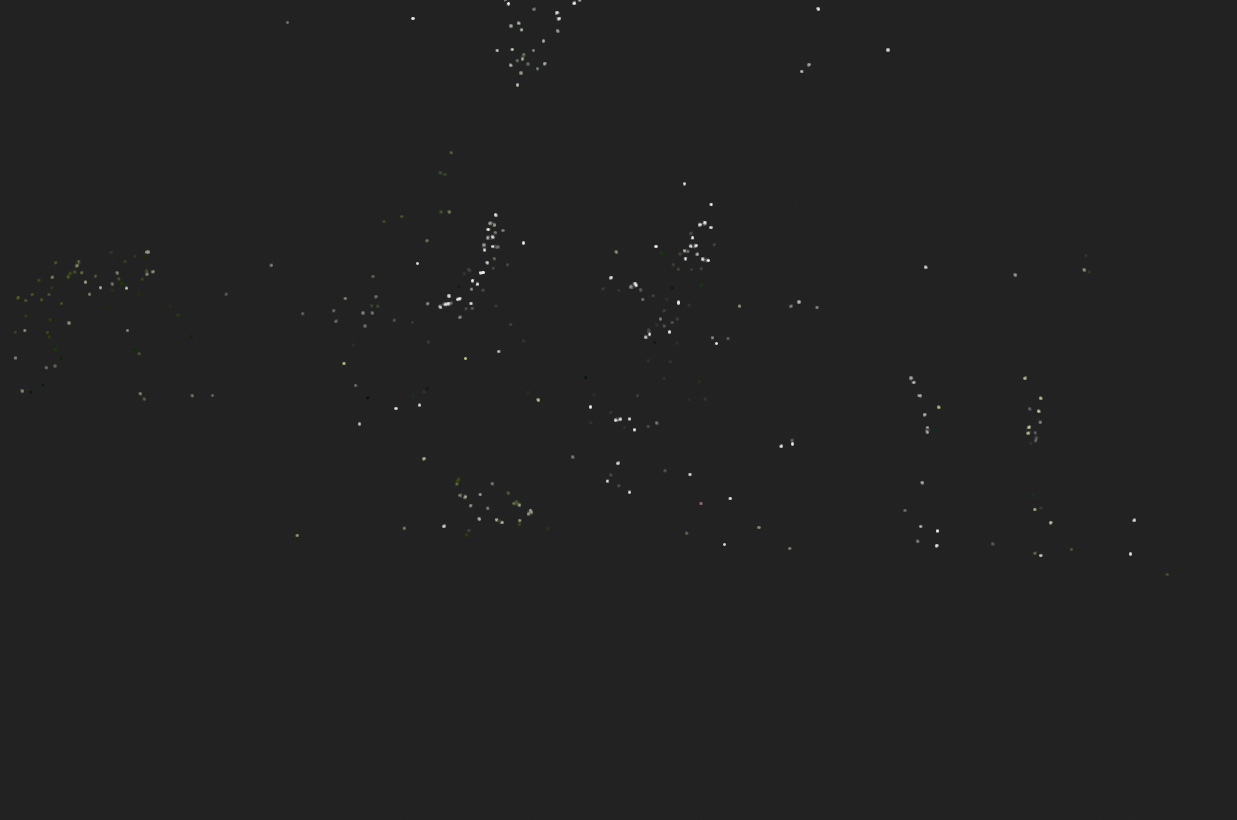
\includegraphics[width=0.98\linewidth]{figures/colmap_pointcloud.png}
  \caption{Point cloud created with COLMAP.}
  \label{fig:pointcloud_colmap}
\end{subfigure}
\caption{Comparison between $\pi^3$ point cloud and COLMAP point cloud, of the bike scene from MipNeRF360 Dataset with 24 training images~\cite{mipnerf360,wang2025pi3,SFM-Original}.}
\label{fig:pointcloud_comparison}
\end{figure}

\subsection{Depth Supervision}
\label{sec:depth_supervision}
From $\pi^3$, we obtain the per view point clouds which can be used as a depth map.
For depth regularization, we evaluated different losses.

Standard L1 and L2 losses often cause the model to overfit to the limited fidelity of the inferred depth maps. We also evaluated the Global-Local Depth Normalization from \textit{DNGaussian}~\cite{DNGaussian} but found it unnecessary given the inherent scale consistency of our predictions. Instead, we utilize a Pearson correlation loss, which has demonstrated superior performance. This approach enforces structural consistency while enabling the recovery of high-frequency details that are missing from the initial depth estimation.
%The Pearson correlation coefficient is defined as:
%\begin{equation}
%    PCC(a,b) = {\frac{\sum^N_{i=1} (a_i-\bar{a})(b_i-\bar{b})}{\sqrt{\sum^N_{i=1}(a_i-\bar{a})^2 \sum^N_{i=1}(b_i-\bar{b})^2}}},
%\end{equation}
%where $\bar{a}$ and $\bar{b}$ are defined as:
%\begin{align}
%    \bar{a}=\frac{1}{N}\sum^N_{i=1}a_i, \quad
%    \bar{b}=\frac{1}{N}\sum^N_{i=1}b_i,
%\end{align}
%where N is the number of samples, $a_i$ and $b_i$ are the i-th sample of $a$ and $b$~\cite{SparseGS}. The Pearson correlation coefficient is +1 when there is a strong positive correlation, meaning that $a$ and $b$ increase together. The coefficient is -1 when there is a strong negative correlation, meaning that high values of $a$ correspond to low values of $b$, and vice versa. The final loss, used for training, is given by $1-PCC(a, b)$.

In addition to the default Pearson correlation loss, we also integrated the confidence given by $\pi^3$. As a result, the final depth can be modeled even more accurately by assigning low weights to uncertain regions.
Our newly created confidence-aware depth loss, $\mathcal{L}_{pearson}$, is defined as:
\begin{equation}
    \mu_p = \frac{\sum^N_{i=1} C_i D^p_{i}}{\sum^N_{i=1} C_i}, \quad \mu_t = \frac{\sum^N_{i=1} C_i D^t_{i}}{\sum^N_{i=1} C_i},
\end{equation}
\begin{equation}
    \bar{D}_p = D_p - \mu_p, \quad \bar{D}_t = D_t - \mu_t,
\end{equation}
\begin{equation}
    \small
    P_{conf} = \frac{\sum^N_{i=1} C_i \bar{D}^p_{i} \bar{D}^t_{i}}{\sqrt{\left(\sum^N_{i=1} C_i \left(\bar{D}^p_{i}\right)^2\right)\left(\sum^N_{i=1} C_i \left(\bar{D}^t_{i}\right)^2\right)} },
\end{equation}
\begin{equation}
    \mathcal{L}_{pearson} = 1- P_{conf},
\end{equation}
$N$ is the number of pixels, $D^p_{i}$ is the predicted depth of the i-th pixel, $C_i$ the confidence of the i-th pixel and $D^t_{i}$ is the ground truth of the i-th pixel, which is the depth estimated by $\pi^3$, and $P_{conf}$ is the confidence-aware Pearson correlation.
The resulting rendered depth after 7,000 iterations with the help of confidence-aware Pearson correlation can be seen in \cref{fig:PCC_Ballroom}.

%\begin{figure}
%\centering
%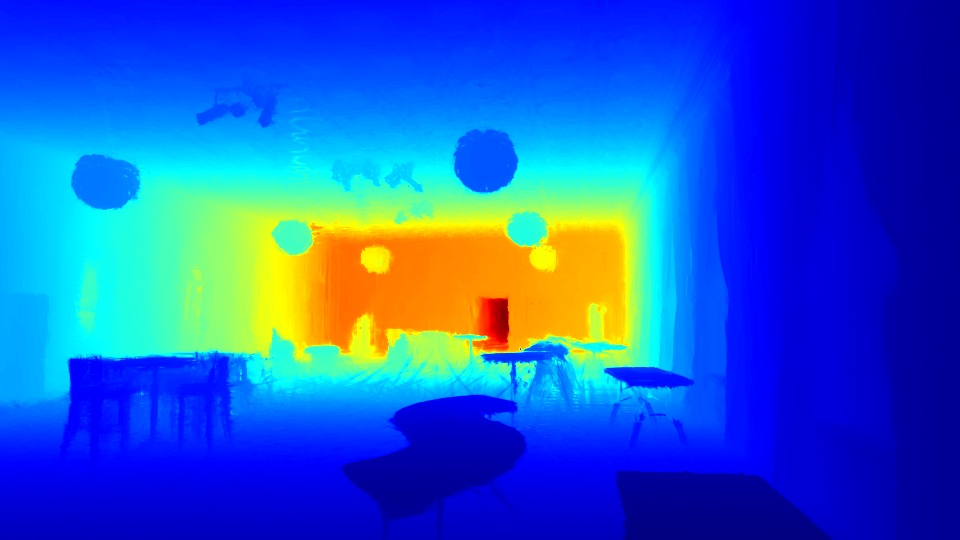
\includegraphics[width=.8\linewidth]{figures/depth_ballroom.jpg}
%\caption{Depth rendering of the Ballroom scene from the Tanks and Temples dataset using the confidence-aware Pearson depth loss~\cite{tankstemples}.}
%\label{fig:PCC_Ballroom}
%\end{figure}

%\begin{figure}
%\centering
%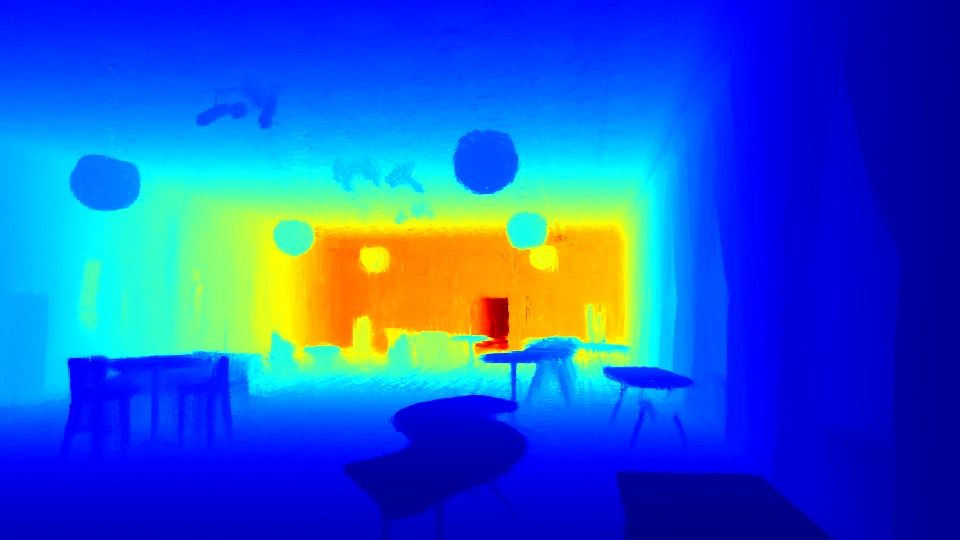
\includegraphics[width=.8\linewidth]{figures/depth_ballroom_default.jpg}
%\caption{Depth rendering of the Ballroom scene from the Tanks and Temples dataset using the Pearson depth loss~\cite{tankstemples}.}
%\label{fig:PCC_Ballroom}
%\end{figure}

\begin{figure}
\centering
\begin{subfigure}{.25\textwidth}
    \centering
    \captionsetup{justification=centering}
    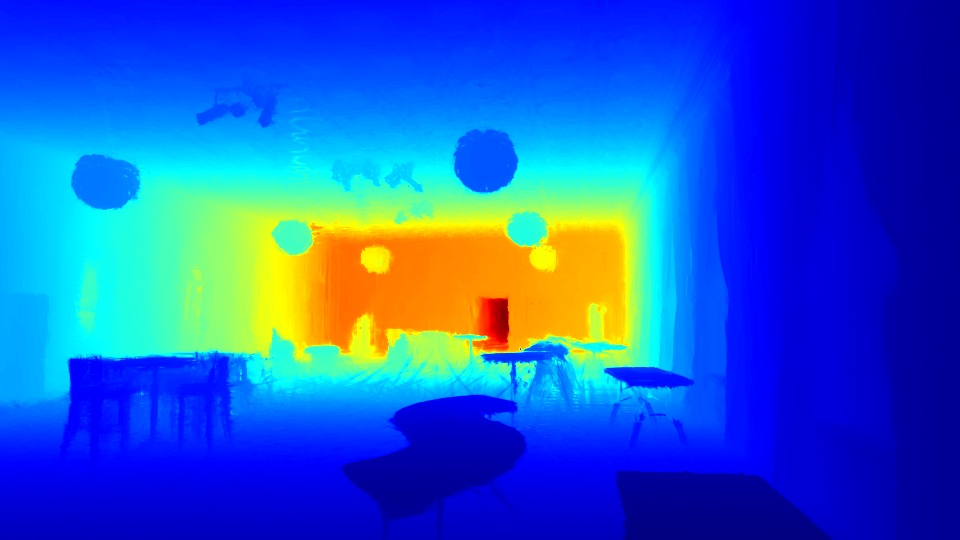
\includegraphics[width=.98\linewidth]{figures/depth_ballroom.jpg}
    \caption{Confidence-aware Peason loss.}
    \label{fig:conf_aware_pearson_depth}
\end{subfigure}%
\begin{subfigure}{.25\textwidth}
    \centering
    \captionsetup{justification=centering}
    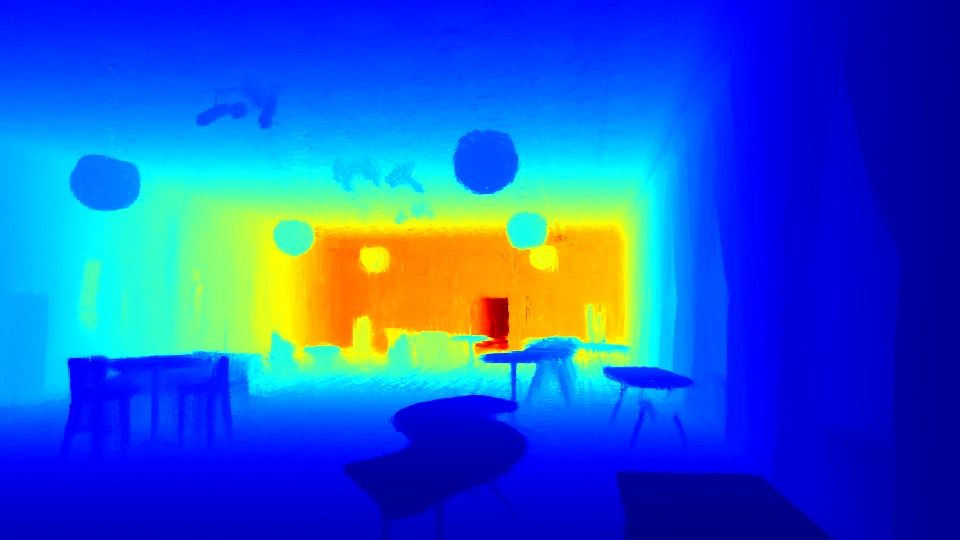
\includegraphics[width=.98\linewidth]{figures/depth_ballroom_default.jpg}
    \caption{Pearson loss.}
    \label{fig:standard_pearson_depth}
\end{subfigure}
\caption{Depth rendering of the Ballroom scene from the Tanks and Temples dataset, comparing the confidence-aware Pearson loss with the standard pearson loss~\cite{tankstemples}. The confidence-aware loss leverages uncertainty estimates to enhance detail, particularly in the background, and also improves performance with low-resolution depth estimates.}
\label{fig:PCC_Ballroom}
\end{figure}

\subsection{Normal Supervision}
\label{sec:normal_supervision}
Surface Normals can be computed with the help of depth maps by calculating the pixel-wise partial derivatives 
$\frac{\partial z}{\partial x}$ and $\frac{\partial z}{\partial y}$, where $x$ and $y$ are the pixel coordinates and $z$ is the depth value, either rendered or estimated by $\pi^3$.
Because $\pi^3$ processes each image in patches of $14 \times 14$ pixels, the gradient is not continuous between adjacent patches, leading to grid-like artifacts, as can be seen in \cref{fig:normal_artifacts}.
To alleviate this problem, we add a mask to ignore these discontinuous regions during loss computation.
The mask is computed by creating a grid with $14 \times 14$ pixel cells, masking the 1-pixel-wide inner border of each cell.
Therefore, the Gaussians are not regularized in these border regions, and the grid artifacts do not appear in the scene representation. The masked normal map can be seen in \cref{fig:normal_masked}.
As supervision, we simply use the L1 loss between the rendered and ground-truth normal map defined as:
\begin{equation}
    \mathcal{L}_{normal}=\frac{1}{N}\sum^N_{i=1}||N^t_{i}-N^p_{i}||_1,
\end{equation}
where N is the number of pixels, $N^t_{i}$ is the ground-truth normal at pixel i and $N^p_{i}$ is the predicted normal at pixel i.

\begin{figure}
\centering
\begin{subfigure}{.25\textwidth}
    \centering
    \captionsetup{justification=centering}
    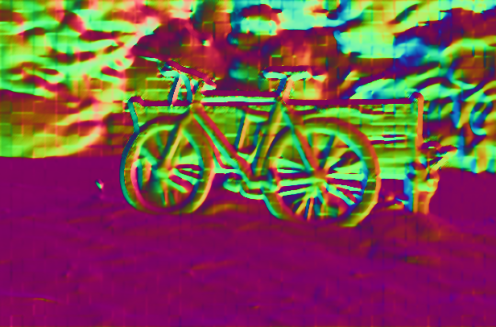
\includegraphics[width=.98\linewidth]{figures/normal_default.png}
    \caption{Default normal map with artifacts.}
    \label{fig:normal_artifacts}
\end{subfigure}%
\begin{subfigure}{.25\textwidth}
    \centering
    \captionsetup{justification=centering}
    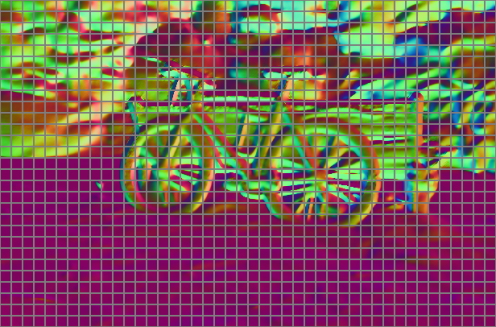
\includegraphics[width=.98\linewidth]{figures/normal_masked_out.png}
    \caption{Masked normal map.}
    \label{fig:normal_masked}
\end{subfigure}
\caption{The Normal map generated from the depth map using partial derivatives, which introduces grid artifacts, and the masked normal map, which removes grid artifacts introduced by $\pi^3$ architecture~\cite{wang2025pi3}.}
\label{fig:normals}
\end{figure}

\subsection{Depth Warping}
\label{sec:depth_warping}

To improve generalization of our model further, we include pseudo-views which are generated with the help of depth warping. This is achieved by projecting the image pixels from one camera into 3D space, and then reprojecting the 3D points into the 2D image plane of a target camera.
For accurate results, we only project pixels with high confidence and mask out the rest, including unseen regions. To generate high-quality pseudo-cameras, we use circle interpolation with the camera parameters as input. A circle can be defined by three points, so we use the two nearest cameras to the target camera for pseudo-view generation. The positions of the three cameras define our circle. Now then interpolate by a certain amount between each pair of neighbouring views, which results in two additional views per camera. We can generate an arbitrary number of pseudo-views by adjusting the interpolation step size. However, in our experiments, two pseudo-views between each pair yielded the best results.
The nearest cameras are already computed by PGSR, therefore we can reuse them. A few examples of these generated pseudo-views can be seen in \cref{fig:reprojection}.
These pseudo-views are then used throughout training for additional supervision with the help of SSIM and L1 loss, but with a weight set to \textit{0.1}.
\begin{figure}
\centering
\begin{subfigure}{.25\textwidth}
    \centering
    \captionsetup{justification=centering}
    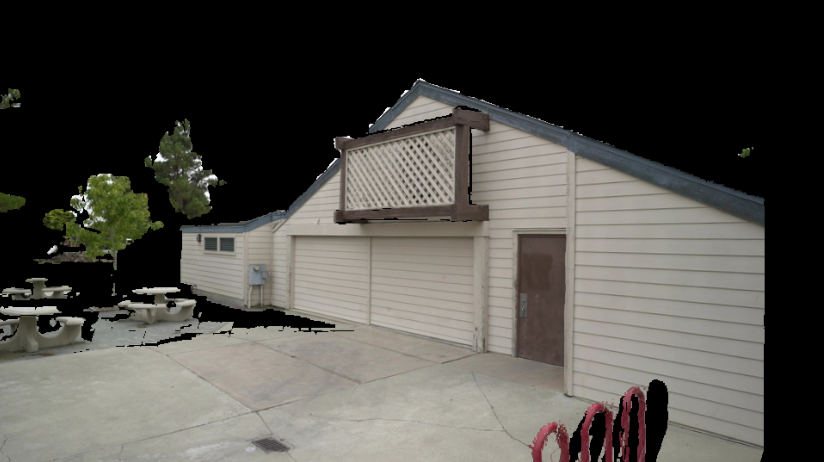
\includegraphics[width=.98\linewidth]{figures/Reprojection1_Barn.png}
    \label{fig:reprojection_1}
\end{subfigure}%
\begin{subfigure}{.25\textwidth}
    \centering
    \captionsetup{justification=centering}
    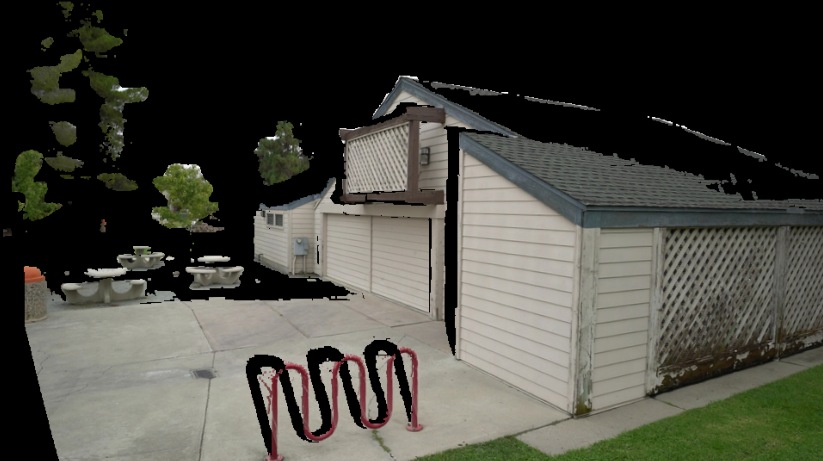
\includegraphics[width=.98\linewidth]{figures/Reprojection2_Barn.png}
    \label{fig:reprojection_2}
\end{subfigure}
\caption{The two Figures show two reprojection examples with the applied mask for the Barn scene of the Tanks and Temples dataset~\cite{tankstemples}.}
\label{fig:reprojection}
\end{figure}